\chapter{Für Nerds}
\label{ch:fuerNerds}
\textit{Die eigene Sammlung auf der eigenen Homepage veröffentlichen. Mit Hilfe von Plugins für OpenCms kein Problem für PUMA.}
\section{URL-Syntax\index{URL-Syntax}}
\label{sec:urlSyntax}
Sie können die Funktionen von PUMA nicht nur über das Menü (\autoref{sec:hauptmenue}) erreichen, sondern auch direkt über die URL ansteuern. Die URL ist die Adresse einer Seite, die im Adressfeld des Browsers eingegeben, bzw. angezeigt wird. Die Seite mit der Adresse \texttt{\begin{small}https://puma.ub.uni-stuttgart.de/user/mueller/forschungsdaten\end{small}} liefert beispielsweise alle Einträge des Benutzers \textit{mueller} zurück, die mit dem Tag \textit{forschungsdaten} gekennzeichnet sind.
Der Teil \texttt{https://puma.ub.uni-stuttgart.de} bezeichnet den Ort der PUMA-Installation, der Rest der URL steuert, welche Seiten oder Inhalte von PUMA zurückgegeben werden. 
 
%nach hinten verschieben
\subsection{Parameter}
\label{subsec:parameter}
Mit einem Fragezeichen können an eine URL noch Parameter angehängt werden, die die Ausgabe steuern (Sortierung, Anzahl angezeigter Einträge). Mehrere Parameter werden durch ein \& getrennt. Die URL \texttt{\begin{small} /user/mueller?items=25\&sortPage=author\&sortPageOrder=desc\end{small}} liefert zum Beispiel die ersten 25 Einträge des Benutzers \textit{mueller} sortiert absteigend nach dem Autor. 

Immer wenn Sie in PUMA eine Liste von Lesezeichen oder Publikationen ausgeben, können Sie diese sortieren, indem Sie an die URL einen oder mehrere der folgenden Suchparameter anhängen. Folgende Parameter stehen Ihnen zur Verfügung:
\begin{description}
    \item [sortPage] Wonach wird sortiert?
    \begin{description}
        \item [author] Autorenname
        \item [editor] Herausgebername
        \item [year] Erscheinungsjahr
        \item [entrytype] Publikationstyp
        \item [title] Titel
        \item [booktitle] Buchtitel (insb. bei Artikel in Sammelbänden)
        \item [journal] Journalname
        \item [school] Universitätsname 
    \end{description}
    \item [sortPageOrder] Reihenfolge der Sortierung
    \begin{description}
        \item [asc] aufsteigend
        \item [desc] absteigend 
    \end{description}
\end{description}

Die Parameter \texttt{items} und \texttt{duplicates} steuern wieviele Einträge mit oder ohne Duplikate angezeigt werden:

\begin{description}		
    \item [items] Wieviele Einträge werden angezeigt\hfill \\
		 Wenn dieser Parameter nicht angegeben ist, werden standardmäßig 20 Einträge angezeigt.
    \item [duplicates] Duplikate\index{Duplikate}
    \begin{description}
        \item [yes] Erlaubt Duplikate in der Lesezeichen/- Publikationsliste
        \item [no] Entfernt Duplikate aus der Ergebnisliste
    \end{description}
\end{description}
%Beispiel: \url{?sortPage=year%\&sortPageOrder=asc\&duplicates=no} \newline
%Beispielkasten einfuegen
%Sortiere nach Erscheinungsjahr (sortPage=~year) aufsteigend (sortPageOrder=~asc) und entferne alle Duplikate (duplicates=~no). \newline
\subsection{Allgemeine Seiten}
\label{subsec:allgemeineSeiten}
\begin{enumerate}
    \item \textbf{/} \newline
    Homepage von PUMA, zeigt die aktuellsten 50 öffentlichen Einträge.
    \item \textbf{/popular} \newline
    Zeigt die 100 häufigsten Einträge der letzten 100.000 öffentlichen Einträge.
    \item \textbf{/IhrBenutzername} \newline
    Ihre persönliche Sammlung.
    \item \textbf{/help\_de} \newline
    Hilfeseite.
     \item \textbf{/myBibTeX} \newline
    Zeigt Ihre gesamte Sammlung im BibTex-Format.
    \item \textbf{/myRelations} \newline
    Zeigt Ihre Konzepte/Relationen.
    \item \textbf{/myDuplicates} \newline
    Zeigt die Duplikaten, die sich in Ihrer eigenen Sammlung befinden.
\end{enumerate}    

\subsection{Administrative Seiten}
\label{subsec:adminSeiten}
\begin{description}
    \item \textbf{/settings} \newline
    Einstellungsseite. Auf dieser Seite können Sie:
    \begin{itemize}
        \item Ihr Profil bearbeiten und Kontoeinstellungen ändern,
        \item einen Benutzer zu Ihrer Gruppe hinzufügen,
        \item Ihren API-Schlüssel finden und einen neuen erzeugen,
        \item Ihr Passwort ändern und
        \item Ihre Daten zwischen BibSonomy und PUMA synchronisieren.
    \end{itemize}
    \item \textbf{/postBookmark} \newline
    Neues Lesezeichen einfügen. Überprüft vorab, ob sich die URL der Seite bereits in der Sammlung befindet.
    \item \textbf{/postPublication} \newline
    Neue Publikation einfügen. 
\end{description}

\subsection{Publikations- und Lesezeichenlisten nach verschiedenen Kriterien erstellen}
\label{subsec:suchenMitUrlSyntax}
PUMA bietet Ihnen die Möglichkeit mit Hilfe der URL ihre Publikationslisten nach verschiedenen Kriterien zusammenzustellen und zu filtern. Möglichke Kriterien sind: Tags, Autor, Publikationsjahr, Benutzername der Person, die den Eintrag gespeichert hat, sowie Freunde- und Gruppennamen. \newline
\newline

\subsubsection{Einträge nach Benutzer}
\label{sss:nachBenutzer}

Um die Einträge eines bestimmten Benutzers aufzulisten, verwenden Sie die Syntax \texttt{/user/<benutzername>}, wobei \texttt{<benutzername>} für den PUMA-Benutzername des gewünschten Nutzers steht. Das Ergebnis kann zusätzlich noch nach Tag gefiltert werden: \texttt{/user/<benutzername>/<tag>}. Mehrere Tags können durch ein + verknüpft werden.

Beispiele:
\begin{itemize}
    \item \textbf{/user/eckert} \newline 
    Zeigt alle öffentlichen Einträge des Benutzers \textit{eckert}.
    \item \textbf{/user/eckert/politik} \newline
    Zeigt alle öffentlichen Einträge mit dem Tag \textit{politik} des Benutzers \textit{eckert}.
    \item \textbf{/user/eckert/politik+menschenrechte} \newline
    Zeigt alle öffentlichen Einträge des Benutzers \textit {eckert} an, die sowohl mit dem Tag \textit{politik} als auch mit dem Tag \textit{menschenrechte} verschlagwortet sind.
\end{itemize}

\subsubsection{Einträge nach Tag\index{Tags}/Schlagwort}
\label{sss:nachTag}
Um alle Einträge aufzulisten, die mit einem bestimmten Tag verschlagwortet sind, verwenden Sie die Syntax \texttt{/tag/<tag>}, wobei <tag> durch das gewünschte Tag ersetzt wird. Mehrere Tags können mit einem + verknüpft werden. 

Beispiele:
\begin{enumerate}
    \item \textbf{/tag/politik} \newline
    Zeigt alle öffentlichen Einträge mit dem Tag \textit{politik} an.
    \item \textbf{/tag/politik+menschenrechte}\newline
    Zeigt alle öffentlichen Einträge an, die sowohl mit dem Tag \textit{politik} als auch mit dem Tag \textit{menschenrechte} verschlagwortet sind.
\end{enumerate}

\subsubsection{Einträge nach Autor\index{Autoren}}
\label{sss:nachAutor}

Um alle Publikationen eines bestimmten Autors aufzulisten, verwenden Sie die Syntax \texttt{/autor/<name>}, wobei <name> durch den Nachnamen des Autors ersetzt wird. Die Liste lässt sich mit Hilfe der Syntax \texttt{/autor/<name>/<tag>} auf bestimmte Tags eingrenzen oder durch \texttt{/autor/<name>/sys:<systemtag>:<wert>} mit verschiedenen Systemtags (siehe auch \autoref{sss:systemtags}) weiter einschränken.

Beispiele:
\begin{enumerate}
    \item \textbf{/author/müller} \newline
    Zeigt alle Publikationen des Autors mit dem Namen \textit{Müller} an.
    \item \textbf{/author/müller/dblp} \newline
    Zeigt alle Einträge des Autors \textit{Müller} an, die mit dem Tag \textit{dblp} versch
    \item \textbf{/author/müller/sys:user:eckert}\newline
    Zeigt alle Publikationen des Autors \textit{Müller} in der Sammlung von \textit{Eckert} an.
    \item \textbf{/author/müller/sys:group:puma} \newline
    Zeigt alle Publikationen des Autors \textit{Müller} in der Sammlung aller Gruppenmitglieder der Gruppe \textit{puma} an. 
\end{enumerate}
\end{description}

Mit dem Systemtag \textit{year} lässt sich das Ergebnis auf ein bestimmtes Erscheinungsjahr oder einen bestimmten Zeitraum beschränken:%muss rausrücken

Beispiele:
\begin{enumerate}
    \item \textbf{/author/hotho/sys:year:2007} \newline
    Zeigt alle Publikationen des Autors \textit{Hotho} aus dem Jahre 2007.
    \item \textbf{/author/hotho/sys:year:2003-2007} \newline
    Zeigt alle Publikationen des Autors \textit{Hotho} zwischen 2003 und 2007.
    \item \textbf{/author/hotho/sys:year:-2005} \newline
    Zeigt alle Publikationen des Autors \textit{Hotho} bis zum Jahr 2005 an.
    \item \textbf{/author/hotho+sys:year:1997-} \newline
    Zeigt alle Publikationen des Autors \textit{Hotho} seit 1997 an.
\end{enumerate}

\subsubsection{Einträge von Freunden} 
\label{sss:vonFreunden}
Um die Einträge Ihrer Freunde (\autoref{sec:freunde}) zu sehen, verwenden Sie die Syntax \texttt{/friends}, für alle Freunde oder \texttt{/friend/<name>} für die Einträge eines bestimmten Freundes. Sie können die Ergebnisse wie gewohnt durch die Angabe von Tags weiter einschränken. 

Sie sehen nur die Einträge, die von Benutzern stammen, auf deren Freundesliste Sie stehen und die von diesen Benutzern für Freunde freigegeben wurden (für Freunde sichtbar).

Beispiele:
\begin{enumerate}
    \item \textbf{/friends} \newline
    Zeigt die für Freunde gekennzeichneten Einträge aller ihrer Freunde.
    \item \textbf{/friend/eckert} \newline
    Zeigt die für Freunde gekennzeichneten Einträge des Benutzers \textit{eckert}. Sie können diese Einträge nur dann sehen, wenn \textit{eckert} Sie als Freund angegeben hat.
    \item \textbf{/friend/eckert/politik} \newline
    Zeit die für Freunde gekennzeichneten Einträge des Benutzers \textit{eckert} an, die mit dem Tag \textit{politik} verschlagwortet wurden. 
    \item \textbf{/friend/eckert/politik+menschenrechte} \newline
    Zeigt die für Freunde gekennzeichneten Einträge des Benutzers \textit{eckert} an, die sowohl mit dem Tag \textit{politik} als auch mit dem Tag \textit{menschenrechte} verschlagwortet sind. 
\end{enumerate}

\subsubsection{Einträge nach Sichtbarkeit}
\label{sss:nachSichtbarkeit}
Um zu sehen, welche ihrer Einträge für wen sichtbar sind, können Sie die Syntax \texttt{/viewable/<sichtbarkeit>} verwenden. Als \texttt{<sichtbarkeit>} sind folgende Ausprägungen möglich:
\begin{description}
  \item[public] Einträge, die öffentlich sichtbar sind
	\item[private] Einträge, die nur für Sie selber sichtbar sind
	\item[friends] Einträge, die für die Benutzer sichtbar sind, die auf ihrer Freundeliste stehen
	\item[<gruppenname>] Einträge, die für die Mitglieder der Gruppe <gruppenname> sichtbar sind
\end{description}  

Die Ergebnisse können mit Hilfe der Syntax \texttt{/viewable/<sichtbarkeit>/<tags>} zusätzlich durch Tags eingeschränkt werden. 

Beispiele:
\begin{itemize}
    \item \textbf{/viewable/public} \newline
    Zeigt alle Ihre Einträge an, die Sie als \enquote{öffentlich sichtbar\index{Sichtbarkeit!öffentlich}} eingestellt haben.
    \item \textbf{/viewable/public/politik} \newline
    Zeigt alle Ihre öffentlich sichtbaren Einträge, die mit dem Tag \textit{politik} verschlagwortet wurden.
    \item \textbf{/viewable/private} \newline
    Zeigt alle Ihre Einträge, die Sie als \enquote{privat sichtbar\index{Sichtbarkeit!privat}} eingestellt haben.
    \item \textbf{/viewable/private/politik+menschenrechte} \newline
    Zeigt alle Ihre Einträge an, die nur für Sie sichtbar sind und sowohl mit dem Tag \textit{politik} als auch mit dem Tag \textit{menschenrechte} verschlagwortet wurden. 
    \item \textbf{/viewable/friends} \newline
    Zeigt alle Ihre Einträge an, die Sie als \enquote{für Freunde sichtbar\index{Sichtbarkeit!Freunde}} eingestellt haben.
    \item \textbf{/viewable/puma} \newline
    Zeigt alle Einträge an, die für die Gruppe \textit{puma} als sichtbar eingestellt wurden.
    \item \textbf{/viewable/puma/politik} \newline
    Zeigt alle Einträge an, die für die Gruppe \textit{puma} sichtbar sind und mit dem Tag \textit{politik} verschlagwortet wurden.
\end{enumerate}


\subsection{Gruppenseiten\index{Gruppen}}

\label{subsec:gruppenseiten}
\begin{enumerate}
    \item \textbf{/groups} \newline
    Zeigt eine Liste aller Gruppen, die es in PUMA gibt.
    \item \textbf{/group/puma} \newline
    Zeigt Ihnen alle Einträge von Mitgliedern der Gruppe \textit{puma} an, wenn Sie Gruppenmitglied sind.
    \item \textbf{/group/puma/politik}\newline
    Zeigt Ihnen alle Einträge mit dem Tag \textit{politik} von Mitgliedern der Gruppe \textit{puma} an, wenn Sie Gruppenmitglied sind.
    \item \textbf{/group/puma/politik+menschenrechte}\newline
    Zeigt Ihnen alle Einträge mit dem Tag \textit{politik} und dem Tag \textit{menschenrechte} von Mitgliedern der Gruppe \textit{puma} an, wenn Sie Gruppenmitglied sind.
    \item \textbf{/relevantfor/group/puma} \newline
    Zeigt Ihnen alle Einträge an,  die für die Teilnehmer der Gruppe relevant sind.
    \item \textbf{/followers} \newline
    Zeigt die neuesten Einträge aller Benutzer, denen Sie folgen. Diese Einträge werden mittels eines Rankings so umsortiert, dass die für Sie relevantesten Einträge ganz oben stehen. 
\end{enumerate}
\subsection{Konzeptseiten}
\label{subsec:konzeptseiten}
\begin{enumerate}
    \item \textbf{/concepts/eckert} \newline
    Es werden Ihnen alle Konzepte\index{Konzepte} des Benutzers \textit{eckert} angezeigt.
    \item \textbf{/concept/user/eckert/psychologie} \newline
    Zeigt alle Lesezeichen und Publikationen des Benutzers \textit{eckert} an, denen das Tag \textit{psychologie} oder eines der Unterschlagwörter des Konzeptes als Tag zugeordnet ist. 
\end{enumerate}
\subsection{Suchseiten}
\label{subsec:suchseiten}
Mit der URL-Syntax \textit{/search...} suchen Sie im Volltext nach einem bestimmten Wort. Es handelt sich dabei nicht um Schlagwörter/Tags. Bei Lesezeichen enthält der Volltext die URL, den Titel und die Beschreibung. Bei Publikationen sind der Titel, die Beschreibung und alle BibTex-Felder enthalten.
\begin{enumerate}
    \item \textbf{/search/politik} \newline
    Zeigt Ihnen alle öffentlichen Einträge an, die im Volltext (nicht in den Schlagwörtern!) das Wort \textit{politik} enthalten. 
    \item \textbf{/search/politik+menschenrechte}\newline
    Zeigt alle öffentlichen Einträge, die im Volltext (nicht in den Schlagwörtern!) das Wort \textit{politik} und das Wort \textit{menschenrechte} enthalten. 
    \item \textbf{/search/politik+-menschenrechte} \newline
    Zeigt alle öffentlichen Einträge an, die im Volltext (nicht in den Schlagwörtern!) das Wort \textit{politik}, aber nicht das Wort \textit{menschenrechte} enthalten. 
    \item \textbf{/search/politik+user:droessler} \newline
    Zeigt alle öffentlichen Einträge des Benutzers \textit{droessler}, die im Volltext (nicht in den Schlagwörtern!) das Wort \textit{politik} enthalten. 
    \item \textbf{/search/politik+menschenrechte+user:droessler}\newline
    Zeigt alle öffentlichen Einträge des Benutzers \textit{droessler} an, die im Volltext (nicht in den Schlagwörtern!) das Wort \textit{politik} und das Wort \textit{menschenrechte} enthalten. 
    \item \textbf{/search/politik+-menschenrechte+user:droessler} \newline
    Zeigt alle öffentlichen Einträge des Benutzers \textit{droessler} an, die im Volltext (nicht in den Schlagwörtern!) das Wort \textit{politik}, aber nicht das Wort \textit{menschnerechte} enthalten. 
    \item \textbf{/mySearch} \newline
    Diese Seite bietet eine Schnellsuche in Ihrer eigenen Sammlung.
\end{enumerate}
\subsection{Umgang mit Duplikaten\index{Duplikate}}
\label{subsec:duplikate}
Auf Gruppenseiten kann es häufig vorkommen, dass Einträge (Publikationen) mehrfach angezeigt werden, wenn innerhalb einer Gruppe zwei oder mehr Benutzer denselben Eintrag in ihrer Sammlung haben.\newline
Falls dies nicht gewünscht ist, kann das Verhalten mittels des Parameters \textit{duplicates} wie folgt angepasst werden:
\begin{enumerate}
    \item \textbf{/group/puma/myown} \newline
    Zeigt alle Einträge der Gruppe \textit{puma} an, die mit dem Tag \textit{myown} annotiert sind (auch Duplikate).
    \item \textbf{/group/puma/myown?duplicates=no} \newline
    Zeigt alle Einträge der Gruppe \textit{puma} an, die mit dem Tag \textit{myown} annotiert sind. Für jedes Duplikat wird nur der erste Eintrag angezeigt.
    \item \textbf{/group/puma/myown?duplicates=merged} \newline
    Zeigt alle Einträge der Gruppe \textit{puma} an, die mit dem Tag \textit{myown} annotiert sind. Für jedes Duplikat werden alle Tags \enquote{aufgesammelt} und aggregiert an einem einzelnen Eintrag angezeigt.
\end{enumerate}


\subsection{Export von Seiten}
\label{exportSeite}
\begin{enumerate}
    \item RSS Feeds\index{RSS}
    \begin{enumerate}
        \item \textbf{/publrss/} \newline
        Zeigt einen RSS-Feed der Publikationen aus dem Inhaltsbereich an.
        \item \textbf{/burst/} \newline
        Zeigt ein BuRST-Feed für die Publikationen aus dem Inhaltsbereich an.
        \item \textbf{/aparss/} \newline
        Zeigt ein RSS-Feed im APA-Format für die Publikationen aus dem Inhaltsbereich an.
    \end{enumerate}
    \item Referenz-Metadaten und Formatierung
    \begin{enumerate}
        \item \textbf{/bib/} \newline
        Zeigt alle Publikationen aus dem Inhaltsbereich im BibTeX-Format\index{BibTex} an.
        \item \textbf{/bib/user/eckert} \newline
        Zeigt alle öffentlichen Publikationseinträge des Nutzers \textit{eckert} im BibTeX-Format an.
        \item \textbf{/endnote/} \newline
        Zeigt alle Publikationen aus dem Inhaltsbereich im EndNote-Format an.
    \end{enumerate}
    \item HTML-Formatierung\index{HTML}
    \begin{enumerate}
        \item \textbf{ /publ/} \newline
        Es wird eine einfache Übersicht angezeigt, in der jeder Eintrag als Zeile in einer Tabelle dargestellt ist.
        \item \textbf{/publ/?notags=1} \newline
        In der einfachen Tabellenübersicht werden die PUMA-Schlagwörter in der HTML-Ausgabe unterdrückt.
        \item \textbf{/publ/user/eckert} \newline
        Es werden die Publikationen des Nutzers \textit{eckert} in Tabellenform dargestellt.
        \item \textbf{ /publ/user/eckert/myown} \newline
        Es werden die Publikationen des Nutzers \textit{eckert}, die unter dem Tag \textit{myown} abgespeichert wurden, in der Tabellenübersicht angezeigt. 
    \end{enumerate}
    \item Semantic Web-Formatierung
    \newline \newline \textbf{/swrc/} \newline
        RDF-Ausgabe gemäß der SWRC-Ontologie.
    
\end{enumerate}

\subsection{URL- \index{URL}oder BibTex-Seiten\index{BibTex}}
\label{subsec:hashSeiten}
\begin{enumerate}
    \item \textbf{/url/398aa54c3aea66c147ad74d3089c0612}\newline
    Zeigt Ihnen alle öffentlichen PUMA-Lesezeicheneinträge der URL mit dem MD5-Hash \textit{398aa54c3aea66c147ad74d3089c0612} an.
    \item \textbf{/url/0fa29f649ff82603a98854e0fbbd2cd1/eckert}\newline Zeigt Ihnen die PUMA-Lesezeicheneinträge des Benutzers \textit{eckert} mit dem MD5-Hash \textit{0fa29f649ff82603a98854e0fbbd2cd1} an.
	\item \textbf{/bibtex/1edc3d2bbf4673d84363a675ee64b49bd}\newline Zeigt alle öffentlichen PUMA-Publikationseinträge mit dem Hashkey\index{Hashkey}\newline \textit{1edc3d2bbf4673d84363a675ee64b49bd} an. Der benutzte Hash ist der Inter-Hash.
    \item \textbf{/bibtex/253aa20e7f5e790b745e604039667c47b/eckert}\newline
    Zeigt den PUMA-Publikationseintrag des Benutzers \textit{eckert} mit dem\newline Hashkey 253aa20e7f5e790b745e604039667c47b an. Der benutzte Hash ist der Intra-Hash. PUMA liefert einen Tag-JSON-Feed, der zu einem BibTeX-Eintrag gehört.
    \item \textbf{/json/tags/bibtex/218a34049610d50537e6e09ce71b65605}\newline Diese URL liefert eine JSON-Ausgabe. Sie enthält alle Schlagwörter, welche in Beziehung mit der Publikation stehen, die dem Inter-Hash \textit{218a34049610d50537e6e09ce71b65605} entsprechen. PUMA bietet die Möglichkeit, eine Publikation anhand ihres BibTex-Schlüssels abzurufen.
    \item \textbf{/bibtexkey/Martin\_2014} \newline
    Liefert Publikationen mit dem BibTex-Schlüssel \textit{Martin\_2014}.
    \item \textbf{/bibtexkey/Martin\_2014/droessler} 
    oder \newline \textbf{/bibtexkey/Martin\_2014+sys:user:droessler}\newline
    Liefert Publikationen mit dem BibTex-Schlüssel \textit{Martin\_2014} des Nutzers \textit{droessler}.
    \item \textbf{/bibtexkey/Martin\_2014+sys\%3Auser\%3Adroessler} \newline
    Zeigt alle Einträge mit dem vorgegebenen BibTex-Schlüssel \textit{Martin\_2014} des Benutzers \textit{droessler} an. Haben Sie mehr als einen Eintrag mit dem gleichen BibTeX-Schlüssel, so erhalten Sie eine Liste aller Treffer.
    \item \textbf{/bibtexkey/journals/jacm/HopcroftU69/dblp} \newline
    Sie können die BibTex-Semantik benutzen, um auf Einträge zu verweisen, die wir von DBLP spiegeln  %, sobald Sie gelernt haben, wie DBLP seine BibTeX-Schlüssel erzeugt. noch nachschauen
\end{enumerate}
\section{Duplikatserkennung\index{Duplikat}} 
\label{sec:duplikat}
Die Dupliktaserkennung von PUMA basiert auf Hashkeys. Durch das Ausfüllen der Pflichtfelder Titel, Autor und Jahr wird an Hand dieser drei Felder ein Hashkey für die Publikation erzeugt. Wird nun eine Publikation zum zweiten mal in die Sammlung eingetragen, vergibt PUMA an diese Publikation den gleichen, schon vorhandenen Hashkey. Das System bemerkt die doppelte Vergabe und kennzeichnet die Publikationseinträge als Duplikate. 


\section{Rest-API\index{Rest-API}}
\label{sec:restApi}
PUMA bietet Ihnen einen Webservice auf Basis des Representational State Transfer (REST) an. \newline
REST ist ein Architekturstil für verteilte Softwaresysteme, bei dem eine einheitliche Schnittstelle die Interaktion erleichtert. Die standardisierte Schnittstelle basiert auf dem HTTP-Protokoll und kann über unterschiedliche Programmiersprachen, die HTTP versteht, angesprochen werden.\newline\newline
\textbf{Mögliche Programmiersprachen:}\newline\newline
\underline{1. Java\index{Java}:}   \newline\newline 
\underline{2. PHP\index{PHP}:}\newline
PUMA-API ist ein Paket aus PHP-Skripten, das einen REST-Client enthält sowie einige Utilities, die hilfreich sind für die Entwicklung einer PHP-Applikation, die mit der PUMA-REST-API interagieren soll. Der REST-Client verwaltet Funktionen, die von der PUMA REST-API angeboten werden.
\newline
Weitere Informationen und Sources finden Sie in dem BitBucket-Repository\footnote{\url{https://bitbucket.org/bibsonomy/restclient-php}}.  
\newline\newline
\underline{3. Python\index{Python}:}\newline
Es gibt einen API Client, um mit Hilfe der Programmiersprache Python\footnote{\url{https://www.python.org/}} Einträge aus PUMA abzurufen. Der folgende Codeabschnitt beispielsweise erstellt eine Liste aus Ihren Publikationen:\newline\newline
%bibsonomy = BibSonomy('YOUR_USERNAME', 'YOUR_APIKEY')
%posts = bibsonomy.getPosts('bibtex')
%# do something with the posts...
%for post in posts:
%print post.resource.title %für bibsonomy für PUMA?
Das REST-API-Repository\footnote{\url{http://dev.bibsonomy.org/maven2/org/bibsonomy/bibsonomy-rest-client/}} und die Benutzung der REST-API\footnote{\url{https://bitbucket.org/bibsonomy/bibsonomy/wiki/documentation/api/REST API}} können Sie unter den Links nachlesen.
\newline
Um auf die API zugreifen zu können benötigen Sie den API-Key. Diesen finden Sie auf der Einstellungsseite unter dem Reiter \enquote{Einstellungen}. 






\section{OAuth}
\label{sec:oAuth}
OAuth\index{OAuth} ist ein etabliertes Protokoll für sichere API-Autorisierung, die es Nutzern ermöglicht, einer dritten Anwendung den Zugriff auf ihre Daten zu erlauben, ohne, dass sie ihre Anmeldeinformationen außerhalb von PUMA angeben müssen. Mit OAuth erhalten sie Zugriff auf PUMA, hierfür müssen sie einen OAuth Consumer Key sowie ein Consumer Secret beantragen. Wie Sie dabei genau vorgehen erfahren Sie in der Onlinehilfe von PUMA.\footnote{\url{https://puma.ub.uni-stuttgart.de/help_de/OAuth}}



\section{JavaScript-Codeschnipsel}
\label{sec:javaScriptCode}
Durch die Verwendung von JavaScript-Codeschnipseln\index{JavaScript-Code} erleichtern Sie Ihren Webseitenbesuchern das Vermerken und Arbeiten mit PUMA, und Sie vergrößern Ihre eigene Reichweite. PUMA macht dies mit ein paar Zeilen JavaScript möglich. Fügen Sie den folgenden Code in Ihre Webseite ein und schon gelangen Besucher mit einem Klick zu PUMA und können dort ganz einfach Lesezeichen und Kommentare hinterlegen.
\begin{figure}[h!]
 \centering
 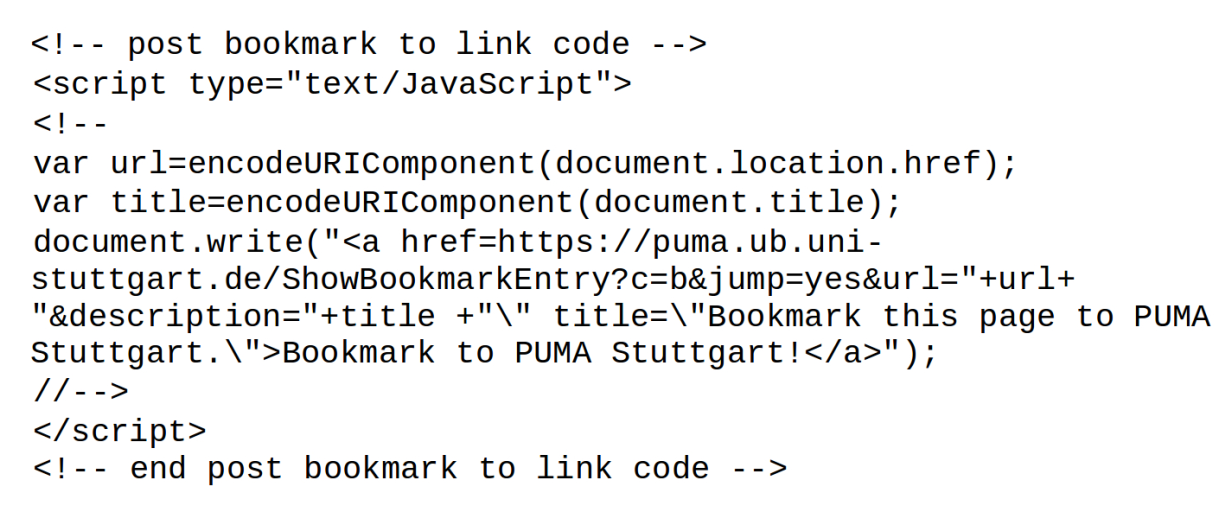
\includegraphics[width=9cm]{Bilder/Kapitel9/JavaScript_Codeschnipsel.PNG}
 \caption{JavaScript-Codesschnipsel}
 \label{fig:javascriptCode}
\end{figure}

\section{Eigenen Webseiten}
\label{sec:eigeneWebseiten}
Es gibt mehrere Möglichkeiten, Inhalte aus PUMA oder Links zu PUMA auf Ihrer eigenen Webseite zu integrieren.

\subsection{Bookmarklinks\index{Bookmarklinks}}
\label{subsec:bookmarklinks}
Einige Webseiten bieten  auf Ihrer Seite einen Bookmarklink an, damit der Benutzer ganz einfach Artikel der Seite in sozialen Netzwerken teilen oder in einem Lesezeichensystem speichern kann. 
\newline Auch PUMA verfügt über einen Bookmarklink, den Sie auf Ihrer eigenen Webseite oder Blog hinzufügen können. Fügen Sie dafür einen kurzen JavaScript-Code\index{JavaScript-Code} ein (dieser befindet sich auf der \enquote{Browser Add-ons \& Bookmarklets Seite}\footnote{\url{https://puma.ub.uni-stuttgart.de/buttons}}) und schon können Ihre Besucher zu Ihren Publikationen und Lesezeichen bei PUMA gelangen.

\subsection{Publikationslisten\index{Publikationslisten}}
\label{subsec:publikationslisten}
Integrieren Sie Publikationslisten\index{Publikationslisten!Eigene Publikationslisten} (z.~B. Ihre eigenen Publikationen), die das gleiche Format haben wie in PUMA, auf Ihrer Webseite. Dazu müssen Sie ein iframe in Ihren HTML-Code\index{HTML} einfügen, das folgendermaßen aussieht:\newline %Screenshot
Die URL kann jede beliebige Seite aus PUMA sein, z.B. Ihre Benutzerseite oder die Seite einer Ihrer Gruppen. 
\begin{figure}[h!]
 \centering
 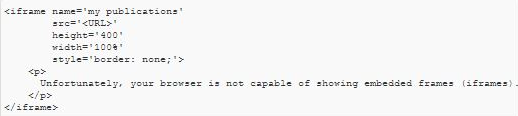
\includegraphics[width=9cm]{Bilder/Kapitel9/HTML-Code.PNG}
 \caption{HTML-Code}
 \label{fig:htmlCode}
\end{figure}
\begin{mdframed}[style=mdfexample1,frametitle={WICHTIG},backgroundcolor=gray!40]Am Ende der URL muss der Parameter \textit{format=embed} steht. Beispielsweise zeigt die URL \url{https://puma.ub.uni-stuttgart.de/user/droessler/myown?items=1000&resourcetype=publication&sortPage=year&sortPageOrder=desc&format=embed}
 alle (bis zu 1000) Publikationen des Nutzers \textit{droessler} an, denen das Schlagwort \enquote{myown} zugeordnet wurde, absteigend nach Jahr sortiert.
\end{mdframed}
\subsection{JSON-Feed\index{JSON-Feed}}
\label{subsec:jsonFeed}
Sie können für jede PUMA-Seite einen JSON-Feed\footnote{\url{http://www.json.org/}} generieren, indem Sie \textit{json/} vor den Pfadteil der URL stellen. Um beispielsweise den JSON-Feed für \textit{/tag/json} zu bekommen, geben Sie \textit{/json/tag/json} ein.

Sie erhalten einen JSON-Feed, der mit Exhibit\footnote{\url{http://www.simile-widgets.org/exhibit/}} kompatibel ist und alle Lesezeichen und Publikationen der entsprechenden Seite enthält. Um den JSON-Feed in Ihr Exhibit einzugeben, fügen Sie einen Link dazu in den Header Ihres Exhibit HTML Codes:\newline
\newline
<link href="https://puma.ub.uni-stuttgart.de/tag/json?callback=cb" type=\enquote{application/jsonp} rel=\enquote{exhibit/data} ex:jsonp-callback=\enquote{cb}%muss noch geschaut werden wegen den " 
\newline
%  Ist von kassel :  Schauen Sie sich diese Liste von Publikationen\footnote{\url{http://www.kde.cs.uni-kassel.de/hotho/publication_json.html}} an, um zu sehen, welche Möglichkeiten Sie mit JSON und Exhibit haben.

\subsection{Zope\index{Zope}}
\label{subsec:zope}
Sie können Inhalte aus PUMA dem Content Management System von Zope\footnote{\url{http://www.zope.org/}} hinzufügen.
\begin{enumerate}
    \item Publikationen\newline
    Publikationslisten können mit Hilfe des PUMA-RSS-Feeds\index{RSS} auf Ihrer Zope-Seite dargestellt werden. Eine detaillierte Beschreibung des RDF Summary Produkts\footnote{\url{http://old.zope.org/Members/EIONET/RDFSummary/}} erhalten Sie bei Zope.
    \item Tagwolken\newline
    Sie haben die Möglichkeit Tagwolken auf Ihren Zope-Seiten zu  erstellen. Eine Anleitung zum Vorgang wird im Folgenden erklärt.
\end{enumerate}
\subsubsection*{Tag-Wolken auf Zope-Seiten} \label{sss:zopeTagwolken}
PUMA-Schlagwörter können auf einer Zope-Seite angezeigt werden. 
\begin{enumerate}
    \item Sie müssen auf eine PUMA-Seite aus Zope heraus zugreifen. Hierfür benötigen Sie das Produkt Kebas Data \footnote{\url{https://sourceforge.net/projects/kebasdata/}}.
    \item Für jede Tag-Wolke, die Sie anzeigen lassen wollen, benötigen Sie ein KebasData-Objekt. Bitte konfigurieren Sie es wie folgt (Benutzername etc. muss entsprechend ersetzt werden):
  
\begin{figure}[h!]
 \centering
 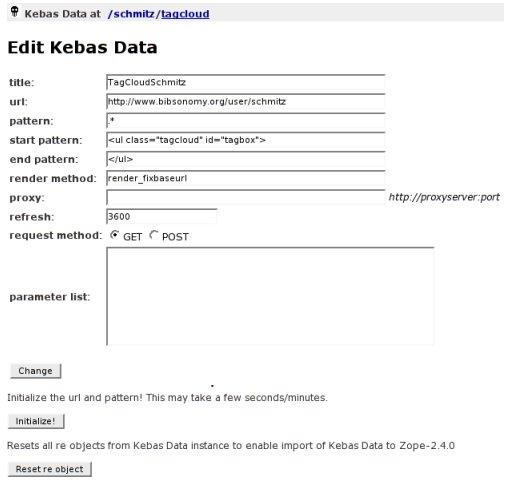
\includegraphics[width=11cm]{Bilder/tag_wolken.jpg}
 \caption{KebayData-Objekt für Tag-Wolken}
 \label{fig:kebayDataObjekt}
\end{figure}

    Es werden nun alle Tags in Ihrer Tag-Wolke angezeigt, die sich zwischen den Start- <ul ...> und den Ende- </ul> Schemata bewegen.
    \item Sie müssen jedoch die von PUMA ausgegebenen URLs überarbeiten, da diese sich auf das PUMA-Hauptverzeichnis und nicht auf Ihre Seite beziehen. Hierfür fügen Sie bitte ein \enquote{Script (Python)}-Objekt namens \textit{render\_fixbaseurl} in Zope an beliebiger Stelle oberhalb des Ordners ein, der Ihre Tag-Wolke enthält. Lassen Sie es zwei Parameter haben und folgendermaßen aussehen: 

    ul = context.match[0]\newline
    ul = ul.replace('href="/', 'href="https://puma.ub.uni-stuttgart.de/')\newline
    print ul\newline
    return printed\newline
    some code block

    \item Für die Anzeige Ihrer Tag-Wolke von \textit{DTML} aus müssen Sie diesen Befehl eingeben: 

    <ul class="tagbox">\newline
        <dtml-var tagcloud>\newline
    </ul> \newline

    \item Für die Anzeige Ihrer Tag-Wolke von einem \textit{Page Template} aus können Sie diesen Befehl benutzen: 

    <ul class=\"tagbox\">\newline
        <div tal:replace="structure here/tagcloud"/>\newline
    </ul>\newline

    \item Nutzen Sie CSS\index{CSS} zur Formatierung der Tag-Wolke nach Ihrem Geschmack. Hier sehen Sie, was wir benutzen; bitte beachten Sie, dass dies die selten vorkommenden Tags verbirgt. Sie können \textit{display: none} durch \textit{display: inline} ersetzen, um deren Anzeige zu aktivieren: 

    ul.tagbox \{ list-style: none; text-align: justify; \}\newline
    ul.tagbox li \{ display: inline; \}\newline
    ul.tagbox li a \{ display: none; text-decoration: none; color: \#e05698; font-size: 60\% \} \newline
    ul.tagbox li.tagone a \{  display: none; text-decoration: none; color: \#a3004e; font-size: 80\% \} \newline
    ul.tagbox li.tagten a \{  display: inline; text-decoration: none; color: \#830030; font-size: 100\% \} \newline
\end{enumerate}

\section{Plugins} 
\label{sec:plugins}
\subsection{OpenCms\index{OpenCms}}
\label{subsec:opencms}
Mit dem OpenCms\index{Plugins!OpenCms} Plugin bei PUMA lassen sich Publikationslisten pflegen und die bibliografischen Daten in anderen Systemen nach nutzen. Ein typischer Anwendungsfall des Plugins ist das Erstellen einer Institutspublikationsliste. Mitarbeiter und/~oder Hilfskräfte des Instituts pflegen die Publikationsdaten in PUMA ein. Die eingetragenen Publikationen können in einer Institutspublikationsliste ausgegeben und auf der Institutswebsite veröffentlicht werden. Hierbei kann zwischen mehreren Zitatiosstil ausgewählt und nach Datum in absteigender oder aufsteigender Reihenfolge sortiert werden. Das Gleiche können die Mitarbeiter ebenfalls für ihre eigenen Publikationsliste machen.
\subsubsection*{Die Umsetzung bei PUMA:}\label{sss:iplPuma}
\begin{enumerate}
\item  Anmeldung auf \url{https://puma.ub.uni-stuttgart.de.}
\item Legen Sie eine Gruppe an.
\item Mitarbeiter und/oder Hilfskräfte des Instituts tragen die Publikationen mit ihrem PUMA-Konto ein und taggen diese mit \textit{for:gruppenname}.
\item Platzieren Sie auf einer Freitextseite in OpenCms den Typ \enquote{Publikationsliste aus BibSonomy/~PUMA} aus dem Typenkatalog.
\item Füllen Sie die Eingabefelder aus.
\end{enumerate}
%\newline\newline
Eine kurze Beschreibung der Eingabefelder:\newline
%\small
\begin{longtabu}{|X|p{7cm}|}\hline
\bfseries Eingabefeld &\bfseries Beschreibung\\ \hline
Titel& 	Der Titel ist frei wählbar und erscheint auf der Seite als Überschrift, z. B. Meine Publikationen. \\ \hline
API-Benutzer­­name &	Der API-Benutzername entspricht dem von Ihnen angegebenen Benutzernamen bei PUMA. Er beginnt nach dem @-Zeichen und erscheint nach dem Login oben rechts im Benutzermenü. API steht für \enquote{Application Programming Interface} (Programmierschnittstelle, über die OpenCms und PUMA Daten austauschen).\\ \hline
API-Schlüssel &	Der API-Schlüs­sel ist ein Zahlencode, den Sie aus Ihrem Benutzermenü unter \enquote{Einstellungen} im Reiter \enquote{Einstellungen} finden und kopieren können.\\ \hline
API-Server &	Der API-Server ist bereits voreingestellt auf \url{https://puma.ub.uni-stuttgart.de/api/}\\ \hline
Quelle & Es kann aus drei möglichen Quellen ausgewählt werden: \textit{user} (Benutzerkonto), \textit{group} (Gruppenkonto) und \textit{viewable} (öffentliche Einträge im System).\\ \hline
Source-ID &	Im Feld Source-ID wird der Benutzer oder Gruppenname eingetragen. Importiert werden also die Daten aus dem jeweils angegebenen Benutzerkonto, z. B. aus dem eigenen oder den öffentlich geteilten Einträgen. Bei \textit{group} sind es dem entsprechend die Daten aus der Gruppe (z. B. schulung).\\ \hline
Tags &	Im Feld Tags (Schlagwörter) werden die Einträge eingegrenzt, die mit diesem Schlagwort vergeben sind. Eine Liste mit den eigenen Publikationen wird mit der Quelle \textit{user}, der Source-ID Benutzername und dem Tag \textit{myown} erzeugt.\\ \hline
Exclude-Tags& An dieser Stelle werden die Schlagwörter eingegeben, zu denen keine Publikationen angezeigt werden sollen.\\ \hline
Search &	Angabe eines Suchbegriffes: Komplette Volltextsuche, auch in hoch geladenen Volltexten. Ausgabe der Publikationseinträge, in denen Suchergebnisse vorkommen.\\ \hline
Anzahl der Publikationen &	Es können bis zu 1.000 Einträge angezeigt werden. Voreingestellt sind 100 Einträge.\\ \hline
Sortierfeld &	Als Sortierfeld kann \textit{none} (keine Sortierung), \textit{author} (der Autor), \textit{entrytype} (der Publikationstyp), \textit{title} (der Titel) oder \textit{year} (das Jahr) gewählt werden.\\ \hline
Sortierreihenfolge &	Definiert die auf (ascending)- oder absteigende (descending) Sortierung.\\ \hline 
Gruppierung &	Gruppierte Ausgabe mit Überschriften. Bei \textit{author} wird nach dem Alphabet (A,B,C, usw.) gegliedert. Bei \textit{entrytype} wird nach dem Publikationstyp (article, book, conference, usw.) sortiert. Mit \textit{title} werden die Publikationen nach dem Anfangsbuchstaben ihres Titels angezeigt, der erste Buchstabe erscheint als Abschnittsüberschrift. Bei \textit{year} werden die Jahreszahlen als Überschriften angezeigt.\\ \hline
Duplikatunterdrückung &	Wenn PUMA einen doppelten Publikationseintrag erkennt, wird nur einer angezeigt.\\ \hline
CSL-Stil &	Im Feld CSL-Stil (Citation Style Language) wird der Zitationsstil ausgewählt, mit dem die Publikationen angezeigt werden sollen. Falls weitere, nicht in der Liste aufgeführte Zitationsstile benötigt werden, können über die CSL-Templates bis zu 7.500 Zitationsstile ausgeben werden.\\ \hline
Zeige Zusammenfassung& 	Das Abstract, falls vorhanden, wird als Link mit ausgegeben.\\ \hline
Zeige BibTex-Code &	Der BibTex-Code kann als Link mit angezeigt werden.\\ \hline
Zeige Link & Der Link zum Volltext wird, falls vorhanden, angezeigt.\\ \hline
\label{tab:eingabefelder}
\end{longtabu}
%\normalsize
Der Inhalt der Eingabefelder für eine Mitarbeiterpublikationsliste und eine Institutspublikationsliste unterscheiden sich. Bei dem folgenden Beispiel beziehen beide Listen die Publikationen aus der Institutsgruppe in PUMA.\newline\newline
\subsubsection*{Beispiel Institutspublikationsliste:\index{Publikationslisten!Institutspublikationslisten}}\label{sss:ipl}
\begin{figure}[h!]
 \centering
 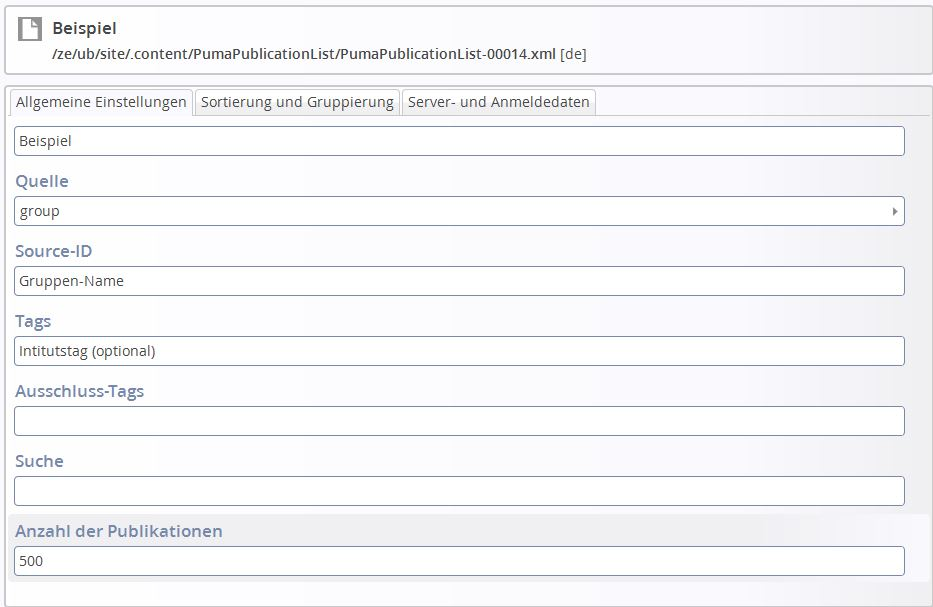
\includegraphics[width=9cm]{Bilder/Kapitel9/Institutsliste1.JPG}
 \caption{Allgemeine Einstellungen}
 \label{fig:iplAllgemeineEinstellungen}
\end{figure}\begin{figure}[h!]
 \centering
 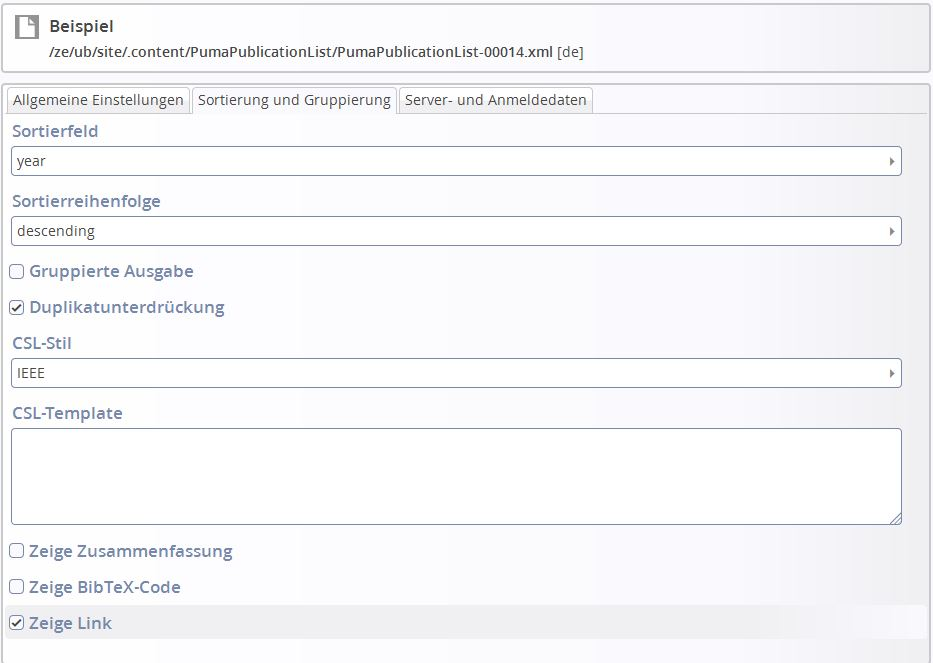
\includegraphics[width=9cm]{Bilder/Kapitel9/Institutsliste2.jpeg}
 \caption{Sortierung und Gruppierung}
 \label{fig:iplSortierungGruppierung}
\end{figure}\begin{figure}[h!]
 \centering
 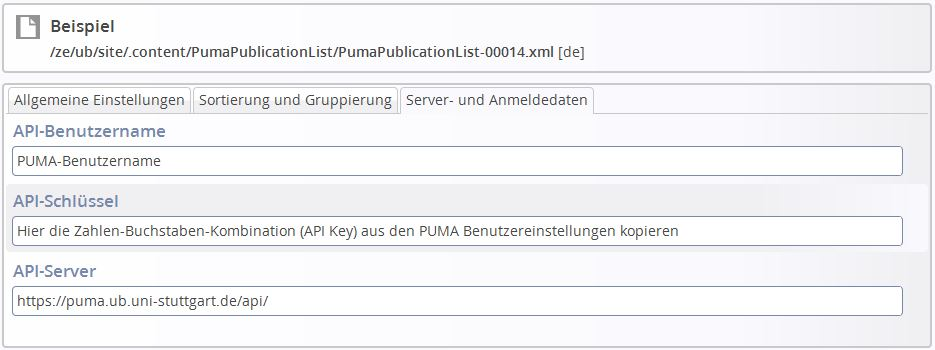
\includegraphics[width=9cm]{Bilder/Kapitel9/Institutsliste3.jpeg}
 \caption{Server- und Anmeldedaten}
 \label{fig:iplServerAnmeldedaten}
\end{figure}
\subsubsection*{Beipiel Mitarbeiterpublikationsliste}\label{sss:mpl}
\begin{figure}[h!]
 \centering
 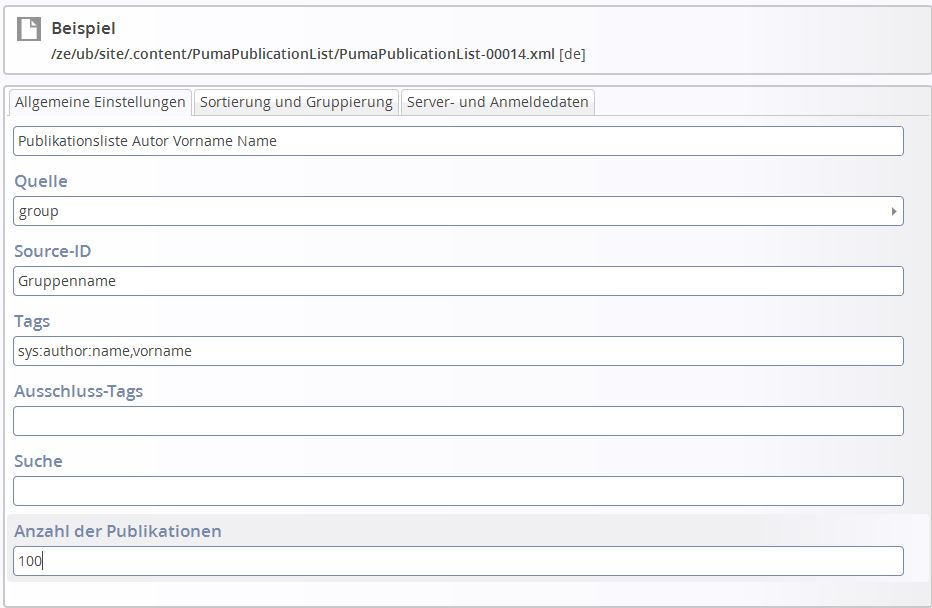
\includegraphics[width=9cm]{Bilder/Kapitel9/Mitarbeiterliste1.jpeg}
 \caption{Allgemeine Einstellungen}
 \label{fig:mplAllgemeineEinstellungen}
\end{figure}
\begin{figure}[h!]
 \centering
 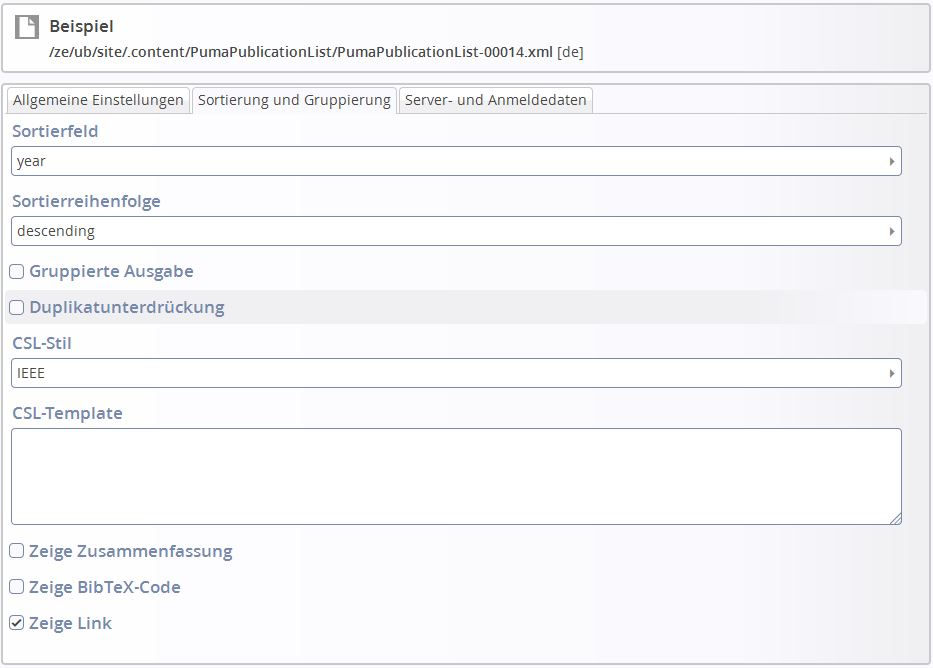
\includegraphics[width=9cm]{Bilder/Kapitel9/Mitarbeiterliste2.jpeg}
 \caption{Sortierung und Gruppierung}
 \label{fig:mplSortierungGruppierung}
\end{figure}
\begin{figure}[h!]
 \centering
 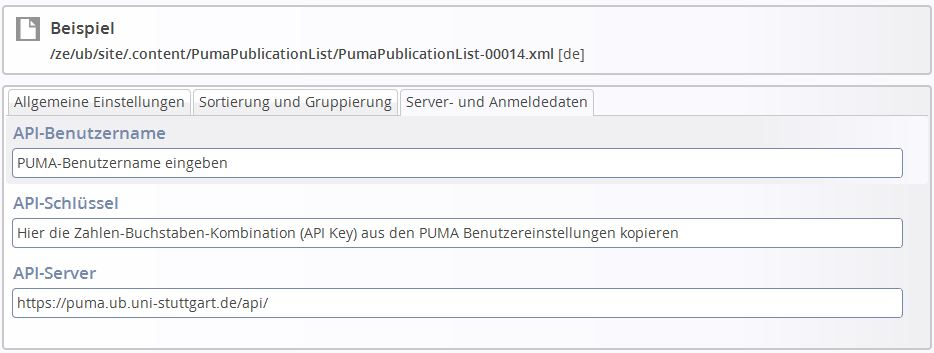
\includegraphics[width=9cm]{Bilder/Kapitel9/Mitarbeiterliste3.jpeg}
 \caption{Server- und Anmeldedaten}
 \label{fig:mplServerAnmeldedaten}
\end{figure}
Wenn die gewünschten Einstellungen veröffentlicht werden, importiert das Plugin die Literatureinträge im ausgewählten Zitationsstil auf die entsprechenden OpenCms-Seite. Veränderungen, die bei PUMA vorgenommen werden, Korrekturen oder weitere Einträge, werden automatisch auf der OpenCms-Seite aktualisiert. OpenCms-Caching-Einstellungen wirken zusätzlich, Änderungen im PUMA-System werden zeitverzögert im OpenCms sichtbar.
\subsection{Typo3\index{Typo3}}
\label{subsec:typo3}
\subsubsection*{Installation}\label{sss:installation}
Um PUMA CSL zu installieren, melden Sie sich bei Ihrer TYPO3-Instanz\index{Plugins!Typo3} als Administrator an. Gehen Sie im Extension Manager zu den Extensions Import results. Suchen Sie nach der Extension ext\_bibsonomy\_csl und importieren Sie diese.
\begin{figure}[h!]
 \centering
 \fbox{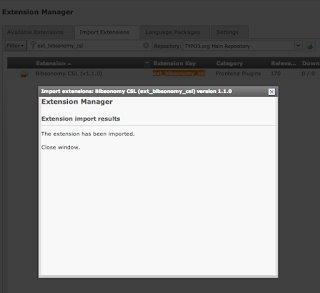
\includegraphics[width=8cm]{Bilder/Kapitel9/extension_manager.jpg}}
 \caption{Extension Manager}
 \label{fig:extensionManager}
\end{figure}
Nach erfolgreichem Import wird die Extension unter \enquote{Available Extensions} angezeigt. Klicken Sie auf das +-Symbol, um es zu aktivieren.
\begin{figure}[h!]
 \centering
 \fbox{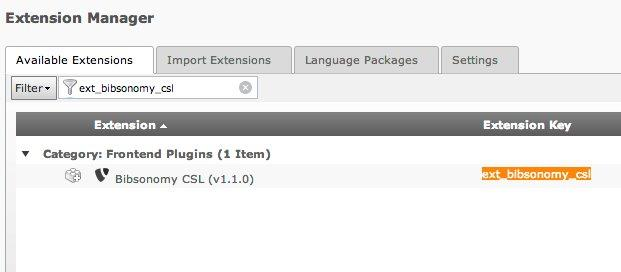
\includegraphics[width=11cm]{Bilder/Kapitel9/available_extensions.jpg}}
 \caption{Available Extensions}
 \label{fig:availableExtensions}
\end{figure}
\newline\newline
\subsubsection*{Publikationslisten hinzufügen mit dem Frontend Plugin}\label{sss:typo3Publikationslisten}
Nachdem Sie die Extension importiert und aktiviert haben, können Sie Publikationslisten erstellen. Fügen Sie dazu der Seite, auf der die Publikationsliste erscheinen soll, ein neues Plugin hinzu. Wählen Sie hierfür aus der Liste \enquote{PUMA Publication List} aus.\newline
\newline
Im Reiter \enquote{General} tragen Sie den Titel für die Publikationsliste ein.
\begin{figure}[h!]
 \centering
 \fbox{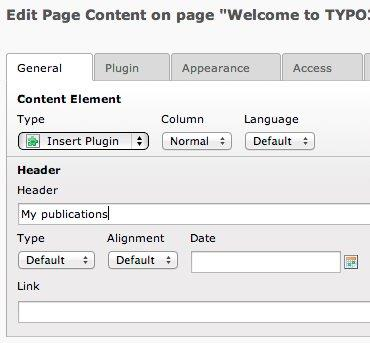
\includegraphics[width=8cm]{Bilder/Kapitel9/reiter_general.jpg}}
 \caption{Reiter General}
 \label{fig:reiterGeneral}
\end{figure}
\newline \newline
Gehen Sie auf den Reiter \enquote{Plugin} und nehmen Sie die gewünschten Einstellungen vor. Sie können zwischen \textit{user}, \textit{group} oder \textit{viewable} wählen, um den entsprechenden Inhalt aus PUMA zu definieren, den Sie in der Publikationsliste haben möchten.\newline
\newline
Beispiel: Sie möchten Ihre eigene Publikationsliste einbinden. Dazu wählen Sie zunächst unter der Rubrik \enquote{Content Source} die Option \enquote{user} aus. Tragen Sie dann den gewünschten (Ihren) Nutzernamen unter \enquote{Insert the id of user, group or viewable source} ein. Anschließend können Sie die Einträge der Publikationsliste über Tags filtern. Geben Sie hierfür die gewünschten Tags in das Feld \enquote{Select content via tags} ein. Um nur eigene Einträge anzeigen zu lassen, verwenden Sie den Systemtag \textit{myown}. Sie können zudem die Anzahl der angezeigten Publikationen begrenzen sowie mittels Freitext filtern.
\begin{figure}[h!]
 \centering
 \fbox{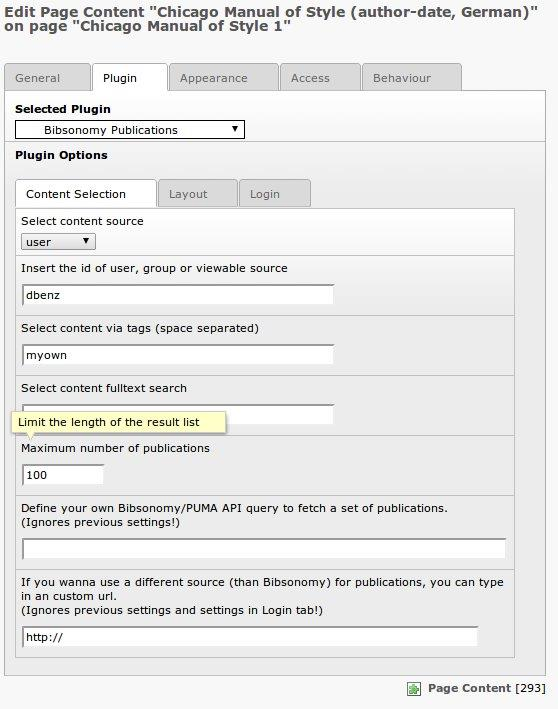
\includegraphics[width=9cm]{Bilder/Kapitel9/reiter_plugin.jpg}}
 \caption{Reiter Plugin}
 \label{fig:reiterPlugin}
\end{figure}

\begin{mdframed}[style=mdfexample1,frametitle={ACHTUNG},backgroundcolor=gray!40]Bitte beachten Sie, dass die Extension Ihre gesamte Publikationsliste darstellt, wie Sie sie in PUMA sehen \textbf{(auch private Publikationen)}. Wenn Sie z.B. an eine Publikation ein Dokument angehängt haben, dann wird dieses auch in der Publikationsliste angezeigt. Dadurch können für Sie \textbf{urheberrechtliche Konsequenzen} entstehen. Wir empfehlen Ihnen daher für die Nutzung einen zusätzlichen Account anzulegen, mit dem Sie in PUMA nur die TYPO3-Publikationen verwalten.
\end{mdframed} 
In der Rubrik \enquote{Layout} können Sie die Gestaltung der Publikationsliste anpassen. Dies geschieht durch Citation Style Language (CSL\index{CSL}), das ist eine frei verfügbare XML-basierte Auszeichnungssprache. Eine große Liste an frei verfügbaren CSL-Vorlagen finden Sie hier: \url{http://www.zotero.org/styles/}.
\begin{figure}[h!]
 \centering
 \fbox{
\includegraphics[width=7cm]{Bilder/Kapitel9/csl_typo.jpg}}
 \caption{Citation Style Language(CSL)}
 \label{fig:csl}
\end{figure}

In der letzten Rubrik \enquote{Login} müssen Sie Ihre PUMA API-Daten\index{API} hinterlegen. Nur so kann sich die TYPO3 Extension bei PUMA anmelden und Ihre Daten abrufen. Ihre API-Daten finden Sie, wenn Sie über das Personensymbol in die Einstellungen gehen und im Reiter \enquote{Einstellungen} nach unten scrollen. 
\subsubsection*{Tag-Wolken hinzufügen mit dem Frontend Plugin}\label{sss:typo3Tagwolken}
Sie können Ihren Webseiten nicht nur Publikationslisten hinzufügen, sondern auch Ihre PUMA  Tag-Wolke(Tagcloud). Fügen Sie dazu der Seite, auf der die Tag-Wolke\index{Tag!Wolke} erscheinen soll, ein neues Plugin hinzu. Wählen Sie aus der Liste \enquote{Bibsonomy Tag Cloud}.\newline \newline 
Wie bei \enquote{Publikationsliste hinzufügen} können Sie auch hier zwischen verschiedenen Modi wählen.\newline \newline 
\subsubsection*{CSL Styles mit dem Backend-Module verwalten}\label{typo3CslBackend}
\newline
TYPO3-Extensions werden klassisch in zwei Module unterteilt, dem Frontend- und Backend-Module. Die Frontend-Module \enquote{Publikationsliste hinzufügen} und \enquote{Tag-Wolke hinzufügen} wurden bereits erklärt. In diesem Abschnitt soll es um das Backend-Modul gehen, mit dem Sie die CSL-Stylesheets verändern können.\newline \newline
Bereits mit der Extension-Installation werden Ihnen eine Reihe von CSL-Stylesheets ausgeliefert. Um weitere Stylesheets hinzuzufügen, erstellen Sie einen neuen Ordner im Seitenbaum und nennen diesen \textit{CSL Styles}. Wählen Sie anschließend diesen Ordner aus. Klicken Sie auf \enquote{Neu} und wählen \enquote{Add a custom style}.\newline \newline
Um ein neue Stylesheets hinzuzufügen gibt es drei unterschiedliche Möglichkeiten:
\begin{enumerate}
\item Geben Sie den XML-Quellcode direkt in das Textfeld ein und klicken Sie anschließend auf \enquote{Save}.
\item Geben Sie in das Textfeld die URL des CSL-Stylesheets ein und klicken Sie auf \enquote{Import}.
\item Laden Sie ein CSL-Stylesheet von Ihrem Computer hoch und klicken Sie auf anschließend auf \enquote{Upload}. 
\end{enumerate}
\begin{figure}[h!]
 \centering
 \fbox{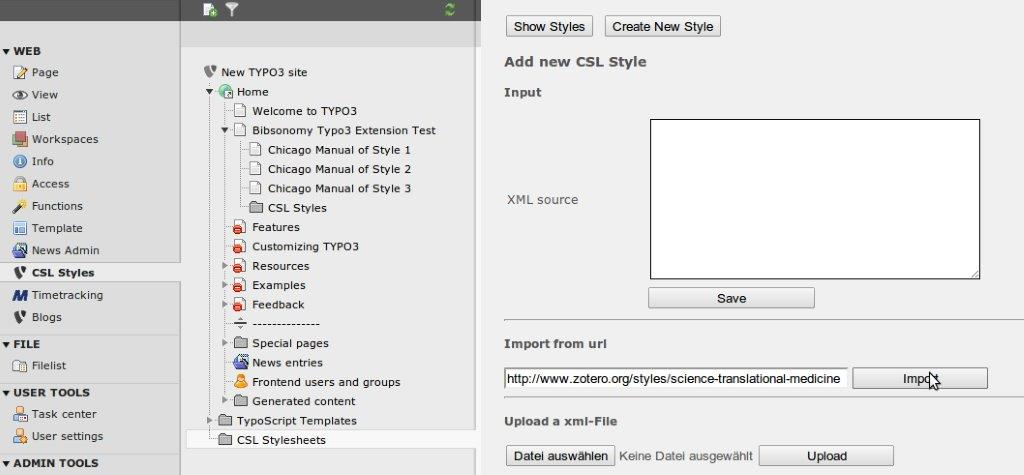
\includegraphics[width=11cm]{Bilder/Kapitel9/stylesheets.jpg}}
 \caption{Neue Stylesheets hinzuzufügen}
 \label{fig:neueStylesheets}
\end{figure}
Um eine Vorschau zu erhalten, klicken Sie auf \enquote{Show Styles}.\newline
Um eine CSL-Stylesheet zu löschen klicken Sie wie gewohnt auf das Mülleimersymbol in Typo3. 
\begin{figure}[h!]
 \centering
 \fbox{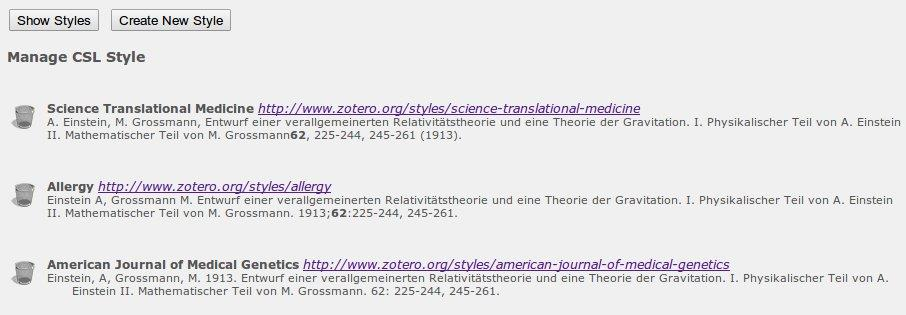
\includegraphics[width=11cm]{Bilder/Kapitel9/csl_stylesheet.jpg}}
 \caption{CSL-Stylesheet löschen}
 \label{fig:cslLoeschen}
\end{figure}
\subsection{WordPress\index{WordPress}}
\label{subsec:wordpress}
Das WordPress-Plugin\index{Plugins!WordPress} ermöglicht Ihnen verschiedene PUMA-Funktionen für Ihren eigene WordPress-Blog zu nutzen.\newline\newline
\textbf{Die Funktionen:}
\begin{enumerate}
   \item Fügen Sie Publikationslisten in einen Artikel ein, indem Sie die Meta-Box-Integration nutzen
    \item Sie können alternativ die WordPress-Shortcodes nutzen
    \item Wählen Sie Ihre Publikationen aus verschiedenen Inhaltstypen aus (z.~B. user/group/viewable)
    \item Filtern Sie die Ergebnisse mit Tags oder einer Volltextsuche
    \item Wählen Sie Ihren bevorzugten Zitierstil (Citation Style Language (CSL))\footnote{\url{ http://citationstyles.org/}}  aus einer Liste aus vorinstallierten Stilen aus
    \item Sie können Ihren eigenen Zitierstil mit Hilfe der CSL\index{CSL} nutzen oder erstellen, um Ihre Literaturliste anzeigen zu lassen
    \item Sie können das Layout Ihrer Liste mit CSS bearbeiten
    \item Speichern Sie Ihre API-Einstellungen (z.B. API-Nutzer, API-Key) auf einer separaten Optionsseite für Administratoren
    \item Fügen Sie Ihrem Blog Tagwolken aus PUMA hinzu und wählen Sie zwischen drei verschiedenen Layouts aus
    \item Stellen Sie Dokumente, die an Publikationen angehängt worden sind, zum Download bereit
\end{enumerate} 
Um Publikationslisten basierend auf der Citation Style Language zu erstellen wird das WordPress-Plugin benötigt. Unter folgender Website kann das Plugin installiert werden: \url{https://wordpress.org/plugins/bibsonomy-csl/}. Eine Anleitung zur Installation finden Sie im BibSonomy Blog \footnote{\url{http://blog.bibsonomy.org/2012/12/feature-of-week-add-publication-lists.html}}
%\subsection{Ilias}
%\label{subsec:ilias}
%\subsection{Moodle}
%\label{subsec:moodle}
%Das PUMA/BibSonomy Module (PBM) ist das PUMA/BibSonomy Plugin für Moodle. Es ermöglicht das Veröffentlichen von Publikationslisten aus PUMA heraus in einen Moodlekurs. Der Zitationsstil, in welchem die Publikationen in Moodle angezeigt werden sollen, kann mit Hilfe des CSL\footnote{\url{http://citationstyles.org/}} festgelegt werden.\newline\newline
%\textbf{ Der Administrator}\newline
%Die folgenden Schritte sind wichtig für die Installation des PBM Plugins: 
%\begin{enumerate}
	%\item Laden Sie sich das Plugin als \*.zip Datei herunter. Wählen Sie auf der Seite von Moodle (\url{https://moodle.org/plugins/view.php?plugin=mod_pbm} ) den Reiter \enquote{Version} aus und klicken auf Download.
	%\item Entpacken Sie die \*.zip Datei im  richtigen Ordner (z.B. /var/www/moodle/mod/pbm)
	%\item Gehen Sie auf die Moodle Webseite und loggen Sie sich als Administrator ein. Gehen Sie unter Einstellungen auf \enquote{Website-Administration} wählen Sie \enquote{Plugins} aus. Klicken Sie anschließend auf\enquote{Plugin-Übersicht}.
	%\item Klicken Sie oben auf der Überblickseite der Plugins auf den Button \enquote{Alle verfügbaren Updates überprüfen}.
	%\item Moodle informiert Sie darüber, dass das Database Update durchgeführt wurde. Bestätigen Sie dies.     
	%\item Sie werden nach einer voreingestellten Serveradresse gefragt, nach Ihren OAuth Consumer-Daten und Ihrer Wahl des Zitationsstils.      
%\end{enumerate}   
%Für die Konfiguration füllen Sie bitte folgende Felder aus:\newline\newline   
%\textbf{Default PBM Server:} Fügen Sie in dieses Feld die URL von PUMA Stuttgart ein (\url{https://puma.ub.uni-stuttgart.de/}). Diese wird ab sofort als Standard verwendet, wenn ein PBM zum Moodle-Kurs hinzugefügt wird.\newline\newline
%\textbf{Comsumer-Key/Consumer-Secret(Optional):}Der Administrator eines Moodle-Kurses kann in den lokalen Administrations-Einstellungen eine OAuth -Nutzer- Bestätigung erstellen. Diese wird dazu verwendet, um die Accounts der Nutzer über die OAuth Authentifizierung mit PUMA zu verknüpfen. \newline\newline
%\textbf{Available CSL files:}Hier können Sie zwischen unterschiedlichen Zitationsstilen auswählen. Weitere Informationen über Zitationsstile gibt es unter \url{http://citationstyles.org/}.
%\newline\newline
%\textbf{Nutzer}\newline
\section{Bitbucket\index{Bitbucket}}
\label{sec:bitbucket}
Bitbucket ist ein auf Git basierendes Versionskontrollsystem, das die Zusammenarbeit mit Teams erleichtert.  
\newline
Bei Problemen oder Fehlern können die Nutzer diese in Bitbucket melden und die Entwickler kümmern sich sofort darum. Hier benötigen die Nutzer ein eigens Bitbucket-Nutzerkonto. Mit diesem melden Sie sich bei Bitbucket an und gehen auf die Bibsonomy/~Puma-Seite\footnote{\url{https://bitbucket.org/bibsonomy/puma}}. Unter dem Reiter \enquote{Issues} können neue Problemmeldungen verfasst werden.
